%!TEX root = ../Thesis.tex

%%%%%%%%%%%%%%%%%%%%%%%%%%%%%%%%%%%%%%%%%%%%%%%%%%%%%%%%%%%%%%%%%%%%%%%%
\chapter{Fundamentals}
\label{sec:fundamentals}
As the section above already focused on the slime mold and Steiner trees, and the subsequent chapters heavily rely on a firm grasp of those topics, it is vital to lay down some fundamentals before going further. Furthermore, it is paramount to understand the basics of graphs and edge bundling, the fundamental concepts of the mathematical definition of Physarium Polycephalum, and the terminology. 

%%%%%%%%%%%%%%%%%%%%%%%%%%%%%%%%%%%%%%%%%%%%%%%%%%%%%%%%%%%%%%%%%%%%%%%%
\section{Graphs}
\label{sec:graphs}

For this thesis, we define a graph as a structure that links unmovable points with lines to allow a representation of relations between objects. In mathematical terms, a graph is defined as $G = (V, E)$, where $V$ are the vertices or nodes and $E$ the edges where $E \subseteq \{\{x, y\} | x, y \in V \text{ and } x \neq y\}$. A graph is either directed or undirected. If a graph is directed, the edges between vertices have a direction; otherwise, they are bidirectional \cite{noauthor_graph_2022}. Important to note is that for calculation purposes, graphs in this thesis are discretized into a grid, which is also a graph. The difference between our grid graph and a regular graph is that all nodes that are not original graph nodes can be moved and deleted.
%%%%%%%%%%%%%%%%%%%%%%%%%%%%%%%%%%%%%%%%%%%%%%%%%%%%%%%%%%%%%%%%%%%%%%%%

\newpage

\begin{figure}[H]
    \centering
    \begin{subfigure}{0.20\linewidth}
        \centering
        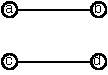
\includegraphics[width=0.9\linewidth]{figures/amb/amb_0.pdf}
        \caption{}
        \label{fig:amb_0}
    \end{subfigure}
    \begin{subfigure}{0.20\linewidth}
        \centering
        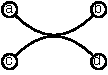
\includegraphics[width=0.9\linewidth]{figures/amb/amb_1.pdf}
        \caption{}
        \label{fig:amb_1}
    \end{subfigure}
    \begin{subfigure}{0.29\linewidth}
        \centering
        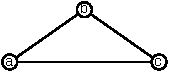
\includegraphics[width=\linewidth]{figures/amb/amb_2.pdf}
        \caption{}
        \label{fig:amb_2}
    \end{subfigure}
    \begin{subfigure}{0.29\linewidth}
        \centering
        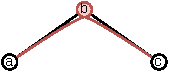
\includegraphics[width=\linewidth]{figures/amb/amb_3.pdf}
        \caption{}
        \label{fig:amb_3}
    \end{subfigure}
    \caption{Graphs \subref{fig:amb_0} and \subref{fig:amb_1} demonstrate the independent edge ambiguity, as in \subref{fig:amb_0} the start and end point of each edge is clearly defined and distinguishable. Still, in the bundled layout in \subref{fig:amb_1}, there is no way to distinguish what connections were made in the original graph. The path endpoint ambiguity is shown in \subref{fig:amb_2} and \subref{fig:amb_3}. As \subref{fig:amb_3} shows, it might be possible to bundle an edge too strong, which could intersect with a node. Images \subref{fig:amb_0} and \subref{fig:amb_1} from \cite{Straub2022}.}
    \label{fig:amb}
\end{figure}

%%%%%%%%%%%%%%%%%%%%%%%%%%%%%%%%%%%%%%%%%%%%%%%%%%%%%%%%%%%%%%%%%%%%%%%%
\section{Bundling Techniques}
\label{sec:bundling_techniques}

Bundling describes a technique that reduces the number of edges and makes a graph visualization more appealing. These results can be archived by bundling paths with similar properties using structures for bundling paths, cluster paths by simulating physical properties, and many more, as seen in \autoref{sec:relatedWork}. This process can reveal high-level patterns and make the graph easier to comprehend.
These graph manipulations also have their drawbacks, as briefly mentioned above. With bundling, the chances for independent edge ambiguities, as shown in \autoref{fig:amb_0} and \autoref{fig:amb_1}, increase, which means that two or more edges get so close to one another that they are no longer distinguishable, and the readability is severely reduced. Bundling approaches can also have path endpoint ambiguities, \autoref{fig:amb_2} and \autoref{fig:amb_3}, such as node-edge overlaps; they occur when the bundling is so firm that the bundled path crosses a node. It is then no longer possible to discern whether the path connects to this node. The last significant ambiguity is edge crossings, as a shallow crossing angle leads to falsely perceived path connections \cite{wallinger_edge-path_2022}.
%%%%%%%%%%%%%%%%%%%%%%%%%%%%%%%%%%%%%%%%%%%%%%%%%%%%%%%%%%%%%%%%%%%%%%%%

\begin{figure}[H]
    \centering
    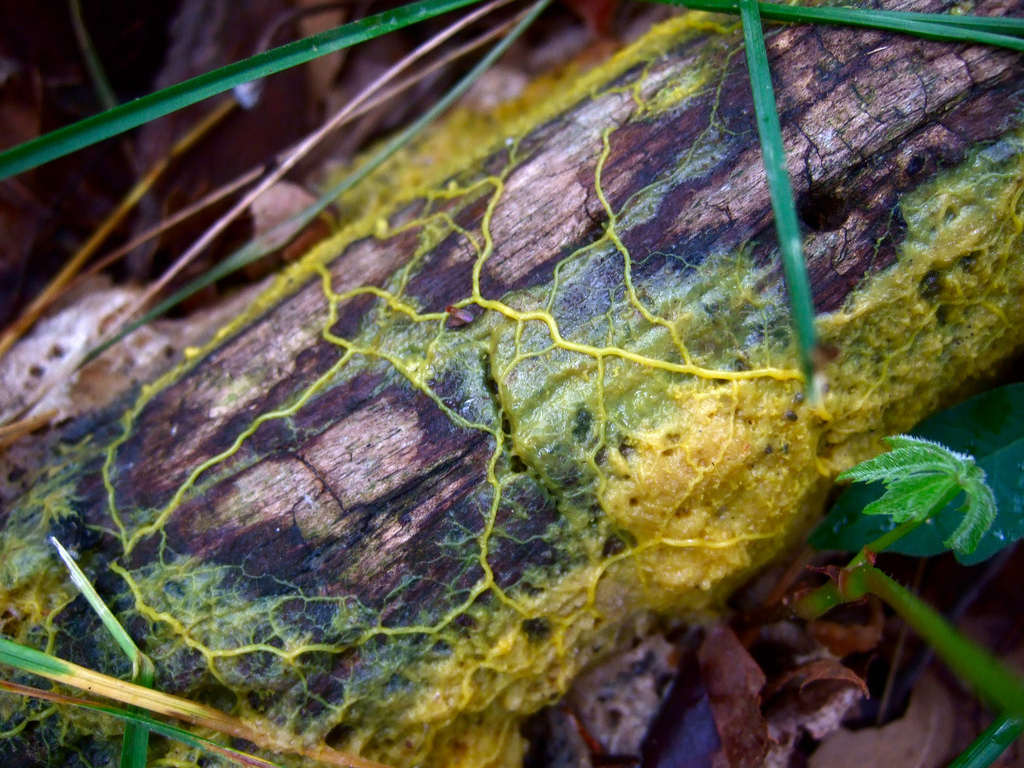
\includegraphics[width=0.75\linewidth]{figures/Physarum_polycephalum_plasmodium.jpg}
    \caption{P. Polycephalum plasmodium (yellow) on tree bark. Easy to spot are the protoplasmic tubes that connect different food sources and parts of the organism \cite{physarium_picture}. These tubes and the processes that control them are the goals of our Physarium approximation algorithm.}
    \label{fig:physarium_picture}
\end{figure}

%%%%%%%%%%%%%%%%%%%%%%%%%%%%%%%%%%%%%%%%%%%%%%%%%%%%%%%%%%%%%%%%%%%%%%%%
\section{Physarium Polycephalum}
\label{sec:polycephalum}

Physarium Polycephalum is a unicellular true slime mold organism that lives on rotten wood and mushrooms, where it can reach a size of multiple square meters. It is, therefore, one of the only cells humans can see with their own eyes and is one of the oldest organisms on earth \cite{jabr_how_2012}. It has a life cycle of four stages, but this thesis will focus only on the plasmodium stage in \autoref{fig:physarium_picture}. In 2000, Nakagaki et al. \cite{nakagaki_maze-solving_2000, nakagaki_path_2001} used this behavior to prove that the slime mold can find the shortest path in a maze. Ten years later, Tero et al. showed that Physarium could solve complicated grids efficiently as the slime mold traced the Tokyo rail system \cite{tero_rules_2010}. The slime mold can also solve the minimal Steiner tree problem in graphs, as Zhang et al. proved \cite{zhang_improved_2014}.

Physarium can archive these results by the ability to move, as the organism constantly searches for new food sources. As mentioned above, this stage is called the plasmodium stage. In this stage, protoplasmic tubes connect to different food sources and circulate nutrients and chemical signals throughout the organism. This tube network can rearrange its structure and continuously contracts to the minimal length, which is the most efficient transport method. The organism finds new food sources through the ability to identify different chemical gradients by using a net-like search structure and following the path with the most robust one. The organism archives mobility by the forward and backward motion of the cytoplasm inside the tubes. This motion is also known as shuttle streaming. Two factors decide the tube efficiency: The first one is the tube diameter which increases or decreases according to the flow. A high flow increases tube diameter, and a low flow rate leads to a decrease. The second one is the length of the tube. A longer tube accelerates the reduction of the diameter \cite{adamatzky2016advances, tero_mathematical_2007}. 

Mathematically this behavior can be described by the pressure difference in two connected vertices and the resulting Poiseuille flow through the edge as the fluid equalizes the pressure \cite{liu_physarum_2015}. The flux in an edge $e_{i,j}$ is described by $Q_{i,j}$, where $D_{i,j}$ denotes the conductivity of $e_{i,j}$, $p_{i}$ and $p_{j}$ are the pressures at $v_i$ and $v_j$, $\xi$ is the viscosity coefficient, and $C_{ij}$ the edge cost. 

\begin{equation}
    \label{eqn:flux}
    Q_{i,j} = \frac{\pi r^{4}_{ij}(p_i-p_j)}{8 \xi C_{ij}} = \frac{D_{i,j}}{C_{i,j}}(p_i-p_j)
\end{equation}

\begin{equation}
    \label{eqn:conductivity_eqn}
    D_{i, j} = \frac{\pi r_{I,j}^{4}}{8\xi}
\end{equation}

After calculating the flux, one vertex is selected as a flow source $v_s$.
With the network Poisson equation \autoref{eqn:poisson_eqn}, it is possible to calculate the pressures in each vertex. 

\begin{equation}
    \label{eqn:poisson_eqn}
    \sum\limits_{i \in V{j}} \frac{D_{i,j}}{C_{ij}}(p_i-p_j) = \begin{cases}
        I_0, \text{ if } j = \text{source}; \\
        -I_0, \text{ if } j = \text{sink}; \\
        0, \text{ otherwise}
    \end{cases}
\end{equation}

However, besides finding efficient paths in networks, Physarium Polycephalum has other interesting properties that researchers can use. For example, the plasmodium stage creates Voronoi diagrams as it expands \cite{shirakawa_simultaneous_2009}; it can learn to anticipate certain events and react before they arrive, and it knows which nutrients it needs for the fastest growth rate \cite{jabr_how_2012}. It can be used as an electric wire to connect components, as Lu and Lopes demonstrated in their study \cite{lu_integrating_2022}.
%%%%%%%%%%%%%%%%%%%%%%%%%%%%%%%%%%%%%%%%%%%%%%%%%%%%%%%%%%%%%%%%%%%%%%%%

%%%%%%%%%%%%%%%%%%%%%%%%%%%%%%%%%%%%%%%%%%%%%%%%%%%%%%%%%%%%%%%%%%%%%%%%
\section{Physarium Network Terms}
\label{sec:network_terms}

As graphs in this thesis are used to simulate fluid networks, it is essential to introduce some specific terms used throughout it. Starting with terminals $T$ where $T \subseteq V$. Terminals are normal nodes in the grid graph at the position of an original graph node. Non-terminal nodes are only created for the calculation of the Steiner points. Other terms that we use in the context of this thesis are sink and source nodes. A source node injects an initial flow $I_0$ into the network. A sink node serves as an outlet for the flow, as in fluid dynamics, the flow conservation has to apply \cite{black_flow_2004}. A Physarium network can have multiple sink or source nodes. How fast the fluid can flow through the network is determined by the conductivity value of the tube, which is dependent on the tube's radius and the fluid's viscosity. The flux is directly related to conductivity, as it describes the amount of fluid flowing through the tube.
%%%%%%%%%%%%%%%%%%%%%%%%%%%%%%%%%%%%%%%%%%%%%%%%%%%%%%%%%%%%%%%%%%%%%%%%

%%%%%%%%%%%%%%%%%%%%%%%%%%%%%%%%%%%%%%%%%%%%%%%%%%%%%%%%%%%%%%%%%%%%%%%%
\section{Steiner Trees}
\label{sec:steinertrees}

\begin{figure}[t]
    \centering
    \begin{subfigure}{0.35\linewidth}
        \centering
        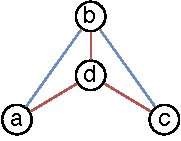
\includegraphics[width=\linewidth]{figures/spannbaum_steiner.pdf}
    \end{subfigure}
  \caption{In blue, a possible minimal spanning tree for the graph $a, b, c$ is drawn; in red, the edges for the Steiner tree, with the node $d$ as a Steiner point.}
  \label{fig:steiner_tree_example}
\end{figure}

Steiner trees, named after the Swiss mathematician Jakob Steiner, were first described in the 19th century. However, their use was limited as the calculation by hand was not feasible for larger graphs. As computers became popular, the approximation of this NP-complete problem became possible, and since then, more and more use cases have emerged. Such as the positioning of telecommunication infrastructure \cite{voss_steiner_2006}, efficiently connecting facility location \cite{eisenbrand_connected_2010}, and other related problems, such as the traveling salesman problem, can also be solved. A compendium of different Steiner tree problems can be found at \cite{Hauptmann_compendium_2015}.

The most relevant problem for this thesis is the Euclidean Steiner tree problem, where the goal is a graph where the total length of the edges is shorter than a minimal spanning tree. In mathematical terms: If $G = (V, E, c)$ is a graph where $c$ is the cost associated with each edge and $N \subseteq V$ is a set of terminals, the Steiner tree is a subgraph $T_G(N)$ of $G$ where every terminal is accessible by a path and the total length of $T_G(N)$ is minimized \cite{byrka_steiner_2013}. The difference to a minimal spanning tree is that Steiner trees can create so-called Steiner points to reduce the overall length of the graph \cite{noauthor_steiner_2022} and are therefore not restricted to the graph edges. A visually easy-to-understand example of the difference between a minimal spanning tree and a Steiner tree can be seen in \autoref{fig:steiner_tree_example}. These Steiner points always have three edge connections and an angle of 120° degrees between each edge. Every Steiner tree with $n$ terminals has a limit of $n - 2$ Steiner points; if all n terminals are leaves, the limit of Steiner points is reached. If a Steiner tree is cut into two new Steiner trees, the new trees will again be a complete Steiner tree. A complete Steiner tree is a Steiner tree with the maximal number of Steiner points. An angle below 120° degrees can not exist in a Steiner tree. Because if it existed, there would be a Steiner point such that the overall length would be smaller, and the 120° angle is given \cite{noauthor_steinerbaumproblem_2021}.
%%%%%%%%%%%%%%%%%%%%%%%%%%%%%%%%%%%%%%%%%%%%%%%%%%%%%%%%%%%%%%%%%%%%%%%%

%%%%%%%%%%%%%%%%%%%%%%%%%%%%%%%%%%%%%%%%%%%%%%%%%%%%%%%%%%%%%%%%%%%%%%%%
\section{Fermat Point}
\label{sec:fermat_point}

We use the Fermat or Torricelli point to move from a discrete to a continuous plot. The Fermat point is the point inside a triangle where the sum of distances to each vertex is minimal. This calculation requires no angles larger than 120° between the vertices. If an angle is greater than 120°, the vertex at the angle becomes the Fermat point. In the context of Steiner trees, the Fermat point has the same conditions as the Steiner point, and it is legit to use this calculation and still expect the results to be Steiner points. 

To calculate the Fermat point, we first have to calculate all angles inside the triangle and check if they are greater than 120°. $A = (x_0, y_0)$, $B = (x_1, y_1)$, $C = (x_2, y_2)$ are the vertices,  $a$, $b$, $c$ are the length of the respected edge, and $\alpha$, $\beta$, $\gamma$ are the angles that are calculated using $y$ and the secant $sec_{\delta}$.

\begin{equation}
    \label{eqn:calculate_angle}
    y = \arccos{\left(\frac{b^2 + c^2 - a^2}{2bc}\right)}
\end{equation}

\begin{equation}
    \label{eqn:calculation_secant}
    sec_{\delta} = \frac{1}{\cos \left(\delta - \frac{\pi}{6}\right)}
\end{equation}

To calculate the position of the Fermat point $F = (x_F, y_F)$, we use $(x_F,y_F)$.

\begin{equation}
    \label{eqn:fermat_position_x}
    (x_F,y_F) = \frac{A_{(x,y)} \cdot a \cdot sec_{\alpha} + B_{(x,y)} \cdot b \cdot sec_{\beta} + C_{(x,y)} \cdot c \cdot sec_{\gamma}}{sec_{\alpha} + sec_{\beta} + sec_{\gamma}}
\end{equation}
%%%%%%%%%%%%%%%%%%%%%%%%%%%%%%%%%%%%%%%%%%%%%%%%%%%%%%%%%%%%%%%%%%%%%%%%